\PassOptionsToPackage{unicode=true}{hyperref} % options for packages loaded elsewhere
\PassOptionsToPackage{hyphens}{url}
%
\documentclass[]{article}
\usepackage{lmodern}
\usepackage{amssymb,amsmath}
\usepackage{ifxetex,ifluatex}
\usepackage{fixltx2e} % provides \textsubscript
\ifnum 0\ifxetex 1\fi\ifluatex 1\fi=0 % if pdftex
  \usepackage[T1]{fontenc}
  \usepackage[utf8]{inputenc}
  \usepackage{textcomp} % provides euro and other symbols
\else % if luatex or xelatex
  \usepackage{unicode-math}
  \defaultfontfeatures{Ligatures=TeX,Scale=MatchLowercase}
\fi
% use upquote if available, for straight quotes in verbatim environments
\IfFileExists{upquote.sty}{\usepackage{upquote}}{}
% use microtype if available
\IfFileExists{microtype.sty}{%
\usepackage[]{microtype}
\UseMicrotypeSet[protrusion]{basicmath} % disable protrusion for tt fonts
}{}
\IfFileExists{parskip.sty}{%
\usepackage{parskip}
}{% else
\setlength{\parindent}{0pt}
\setlength{\parskip}{6pt plus 2pt minus 1pt}
}
\usepackage{hyperref}
\hypersetup{
            pdfborder={0 0 0},
            breaklinks=true}
\urlstyle{same}  % don't use monospace font for urls
\usepackage[margin=1.0in]{geometry}
\usepackage{graphicx,grffile}
\makeatletter
\def\maxwidth{\ifdim\Gin@nat@width>\linewidth\linewidth\else\Gin@nat@width\fi}
\def\maxheight{\ifdim\Gin@nat@height>\textheight\textheight\else\Gin@nat@height\fi}
\makeatother
% Scale images if necessary, so that they will not overflow the page
% margins by default, and it is still possible to overwrite the defaults
% using explicit options in \includegraphics[width, height, ...]{}
\setkeys{Gin}{width=\maxwidth,height=\maxheight,keepaspectratio}
\setlength{\emergencystretch}{3em}  % prevent overfull lines
\providecommand{\tightlist}{%
  \setlength{\itemsep}{0pt}\setlength{\parskip}{0pt}}
\setcounter{secnumdepth}{0}
% Redefines (sub)paragraphs to behave more like sections
\ifx\paragraph\undefined\else
\let\oldparagraph\paragraph
\renewcommand{\paragraph}[1]{\oldparagraph{#1}\mbox{}}
\fi
\ifx\subparagraph\undefined\else
\let\oldsubparagraph\subparagraph
\renewcommand{\subparagraph}[1]{\oldsubparagraph{#1}\mbox{}}
\fi

% set default figure placement to htbp
\makeatletter
\def\fps@figure{htbp}
\makeatother

\usepackage{palatino}
\usepackage{setspace}
\doublespacing
\usepackage[left]{lineno}
\linenumbers

\author{}
\date{\vspace{-2.5em}}

\begin{document}

\hypertarget{environmental-and-genetic-contributions-to-ecogeographic-rules-in-house-mice}{%
\section{Environmental and genetic contributions to ecogeographic rules
in house
mice}\label{environmental-and-genetic-contributions-to-ecogeographic-rules-in-house-mice}}

\vspace{20mm}

Mallory A. Ballinger and Michael W. Nachman\({^\dagger}\)

\vspace{20mm}

Department of Integrative Biology

Museum of Vertebrate Zoology

University of California, Berkeley

Berkeley, CA 94702-3160

\vspace{10mm}

\({\dagger}\) To whom corresponsdence should be addressed:

\href{mailto:mnachman@berkeley.edu}{mnachman@berkeley.edu}

\vspace{40mm}

\textbf{Running title:} Allen's rule and Bergmann's rule in house mice

\newpage

\hypertarget{abstract-200-words}{%
\subsection{Abstract (200 words)}\label{abstract-200-words}}

\newpage

\hypertarget{introduction}{%
\subsection{Introduction}\label{introduction}}

\newpage

\hypertarget{materials-and-methods}{%
\subsection{Materials and Methods}\label{materials-and-methods}}

\newpage

\hypertarget{results}{%
\subsection{Results}\label{results}}

\hypertarget{stonger-evidence-for-bergmanns-rule-figure-1a-than-allens-rule-figure-1b-in-wild-caught-american-house-mice.}{%
\subparagraph{\texorpdfstring{\textbf{1. Stonger evidence for Bergmann's
rule (Figure 1A) than Allen's rule (Figure 1B) in wild-caught American
house
mice.}}{1. Stonger evidence for Bergmann's rule (Figure 1A) than Allen's rule (Figure 1B) in wild-caught American house mice.}}\label{stonger-evidence-for-bergmanns-rule-figure-1a-than-allens-rule-figure-1b-in-wild-caught-american-house-mice.}}

\hypertarget{clear-genetic-basis-for-bergmanns-rule-figure-2a-but-not-allens-rule-figure-2b-in-new-york-and-brazil-house-mice.}{%
\subparagraph{\texorpdfstring{\textbf{2. Clear genetic basis for
Bergmann's rule (Figure 2A) but not Allen's rule (Figure 2B) in New York
and Brazil house
mice.}}{2. Clear genetic basis for Bergmann's rule (Figure 2A) but not Allen's rule (Figure 2B) in New York and Brazil house mice.}}\label{clear-genetic-basis-for-bergmanns-rule-figure-2a-but-not-allens-rule-figure-2b-in-new-york-and-brazil-house-mice.}}

\hypertarget{developmental-plasticity-plays-a-signficant-role-in-shaping-allens-rule-figure-3b-in-american-house-mice.}{%
\subparagraph{\texorpdfstring{\textbf{3. Developmental plasticity plays
a signficant role in ``shaping'' Allen's rule (Figure 3B) in American
house
mice.}}{3. Developmental plasticity plays a signficant role in ``shaping'' Allen's rule (Figure 3B) in American house mice.}}\label{developmental-plasticity-plays-a-signficant-role-in-shaping-allens-rule-figure-3b-in-american-house-mice.}}

\hypertarget{evidence-for-adaptive-plasticity-in-tail-length-figure-4b.}{%
\paragraph{\texorpdfstring{\textbf{4. Evidence for adaptive plasticity
in tail length (Figure
4B).}}{4. Evidence for adaptive plasticity in tail length (Figure 4B).}}\label{evidence-for-adaptive-plasticity-in-tail-length-figure-4b.}}

\newpage

\hypertarget{discussion}{%
\subsection{Discussion}\label{discussion}}

\newpage

\hypertarget{figures-tables}{%
\subsection{Figures \& Tables}\label{figures-tables}}

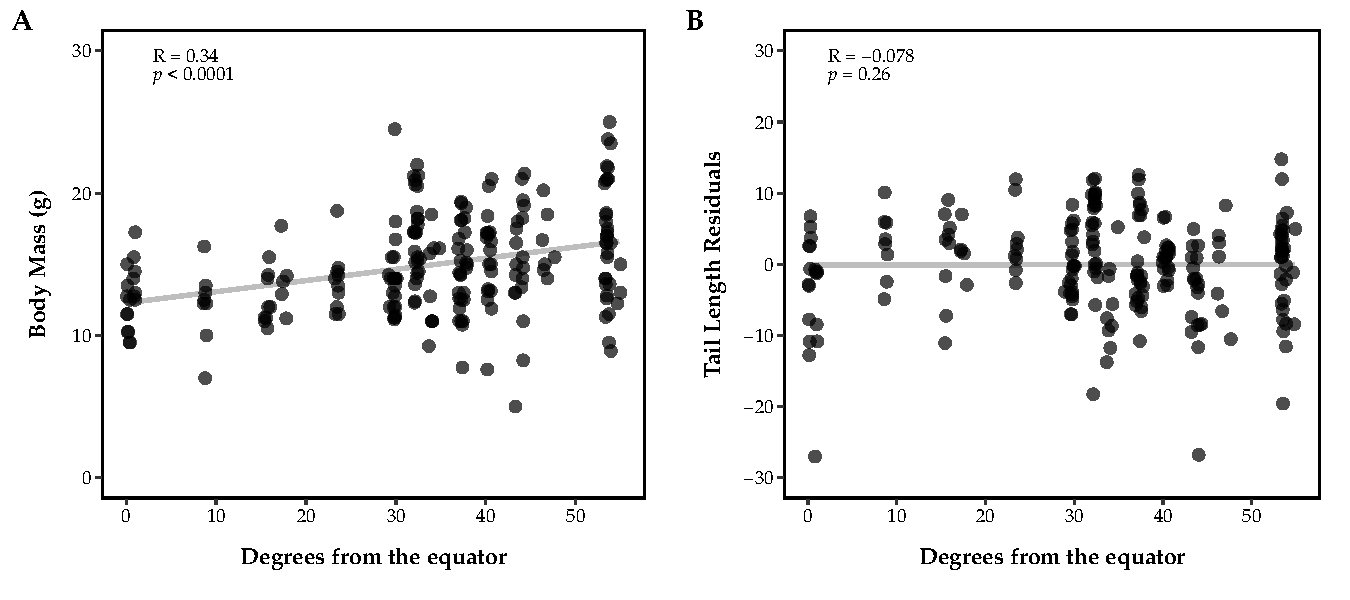
\includegraphics{../figures/Nachman_transects.pdf}

\textbf{Figure 1. The relationship between body weight, tail length, and
absolute latitude in North and South American house mice.} Significant
coorelation between body mass (A) and latitude, but not tail length (B)
and latitude in wild-caught house mice. Tail length residuals were
calculated by regressing tail length from body mass. Both plots include
males and females, with individuals represented as individual point.
Results from Spearman correlations are presented in each plot. Sample
sizes: (A) n = 215; (B) n = 212.

\newpage

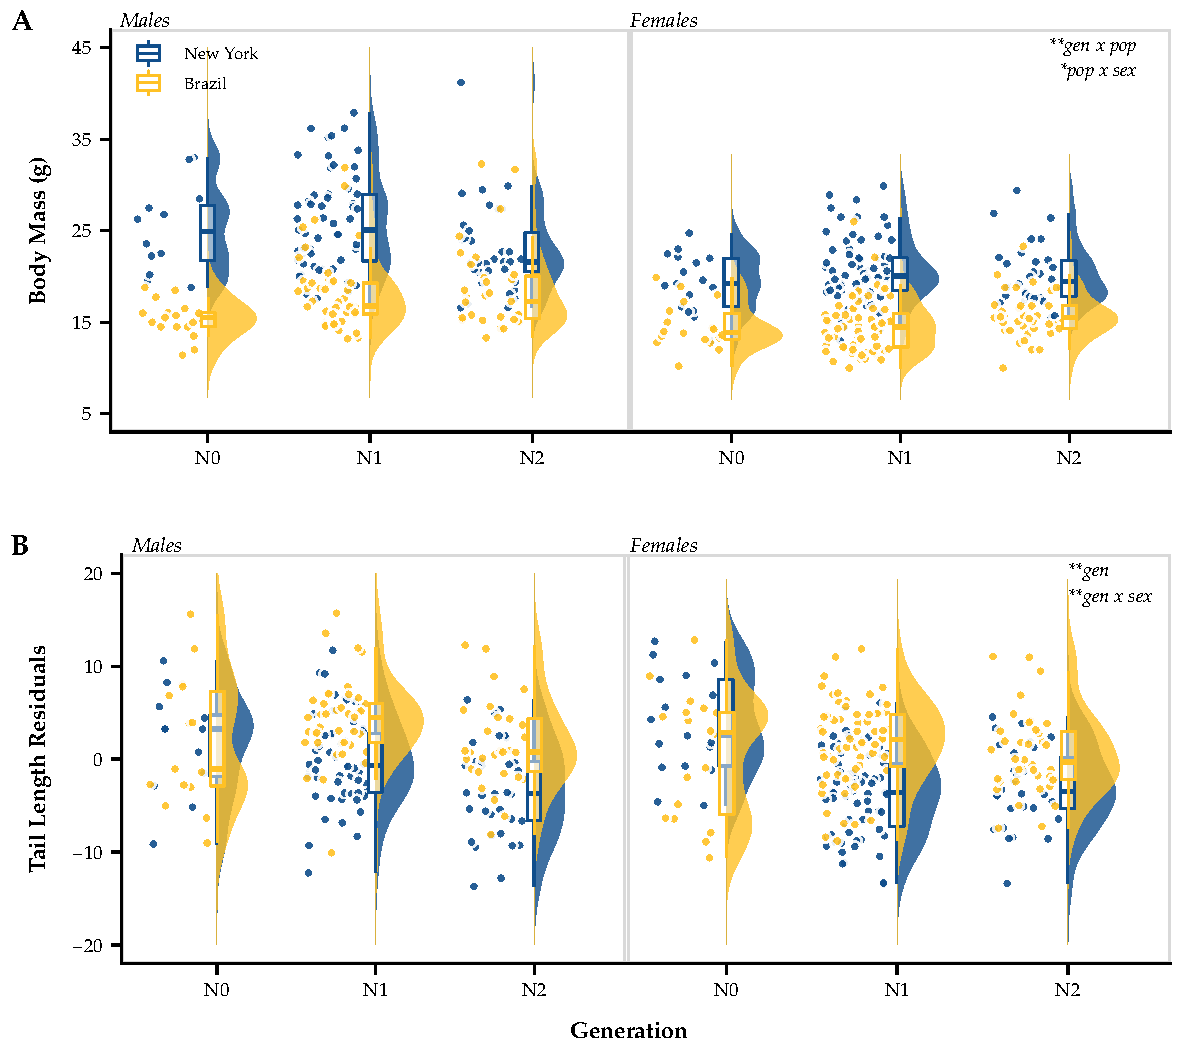
\includegraphics{../figures/generation_phenotypes.pdf}

\textbf{Figure 2. Body mass and tail length differences between
populations and across generations in a common lab environment.} Body
mass differences among populations persist over two generations in lab
(A), indicating a genetic basis. No clear differences in tail length (B)
are seen between populations, suggesting the inherent
``plastic''/``noisy'' nature of tail length. Tail length residuals were
calculated by regressing tail length from body mass. Population-level
data are depticted as boxplots overlayed on density plots, with boxplot
vertical lines denoting 1.5x the inerquartile range. Individuals are
represented as individual points. Results from linear mixed models are
presented in each plot. Only signifiant interactions are depicted in
(A). Sample sizes: (A) n = 438; (B) n = 427. *\emph{P}\textless{}0.05,
**\emph{*P} \textless{}0.01.

\newpage

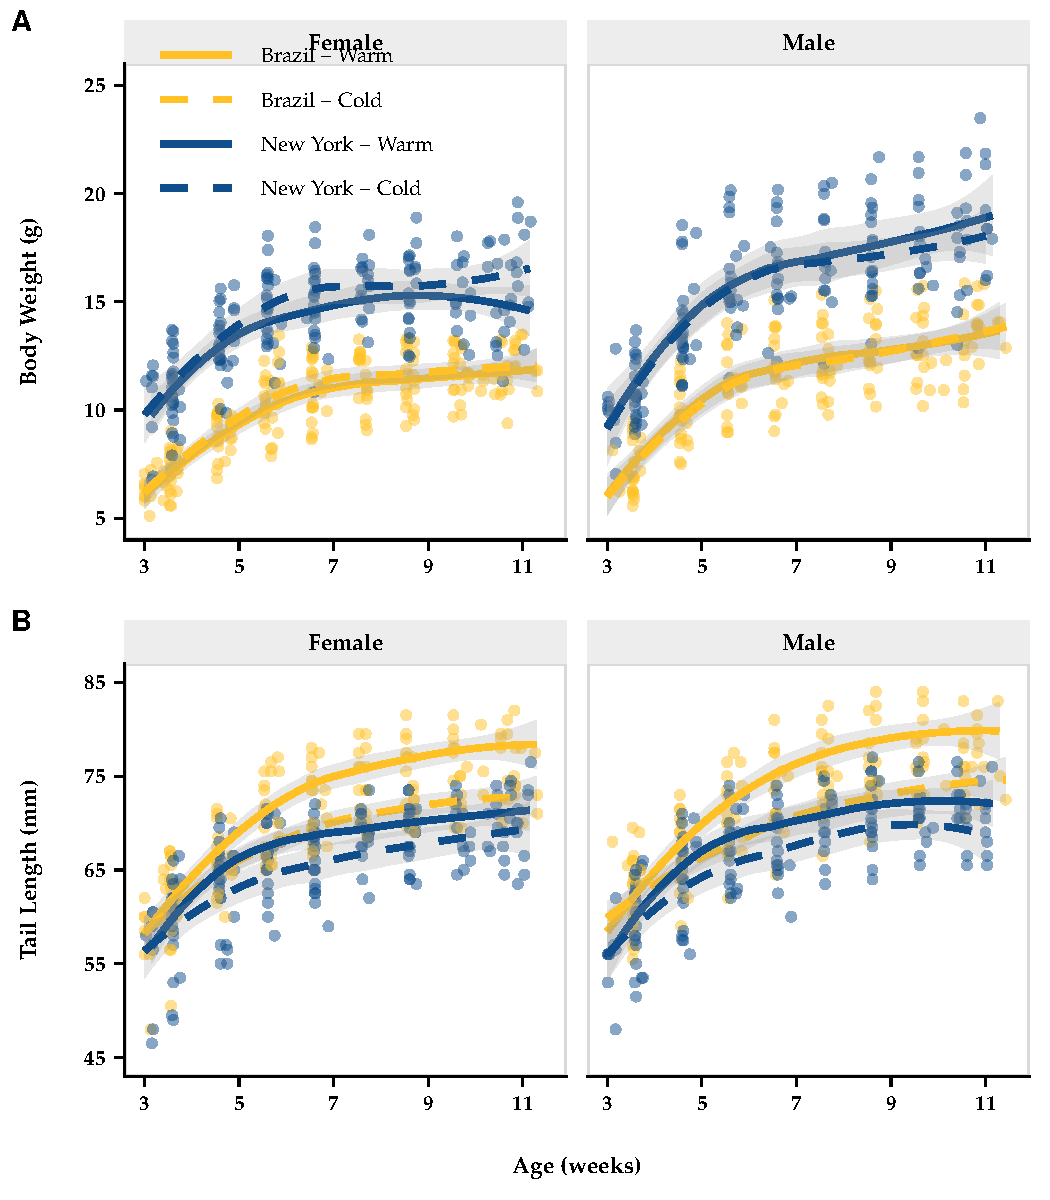
\includegraphics{../figures/weekly_phenotypes.pdf}

\textbf{Figure 3. Body mass and tail length growth trajectories across
environments.} Cold temperatures have very little influence on overall
body mass in New York and Brazil house mice (A). Tail length is highly
influenced by cold temperatures, with cold-housed mice growing shorter
tails compared to warm-housed mice (B). Both New York and Brazil house
mice show plasticity in tail length across development. Individuals are
represented as individual points (n = 80), with population means
depicted as smoothed regression fits, with standard error shading.

\newpage

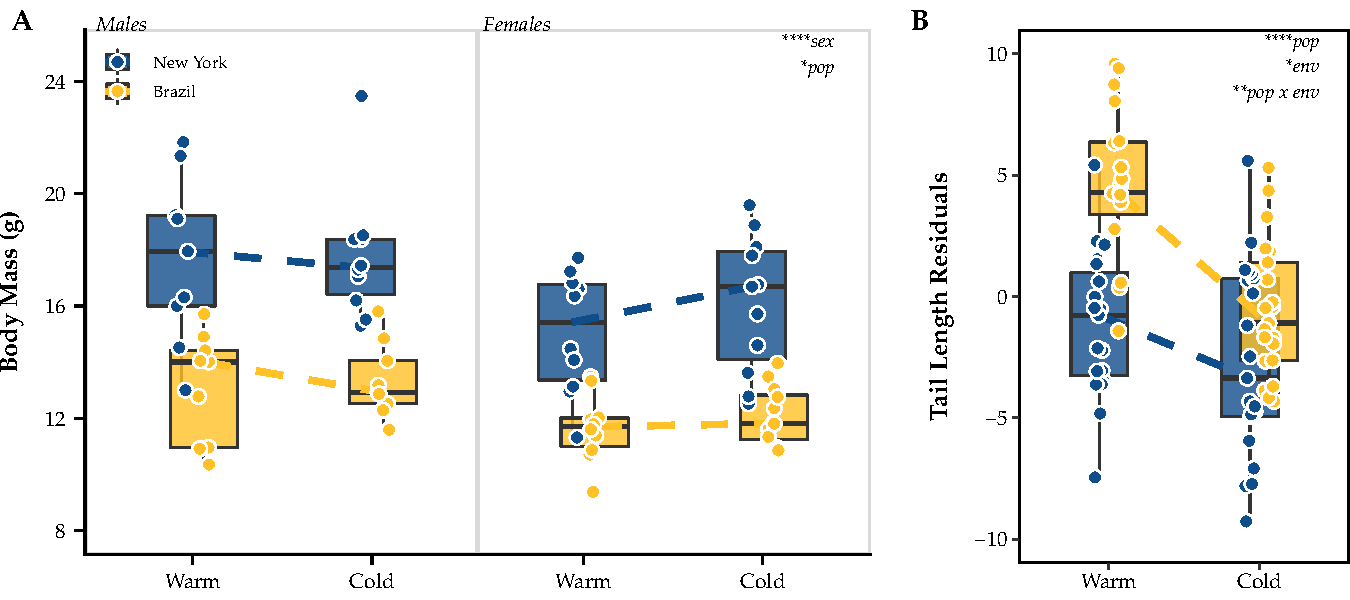
\includegraphics{../figures/RXNs.pdf}

\textbf{Figure 4. Evolved and plastic phenotypic variation among New
York and Brazil house mice.} Very little plasticity in body mass in New
York and Brazil house mice (A). Tail length is highly plastic in both
populations, with tails growing shorter in the cold (B). Brazil house
mice show adaptive plasticity in tail length. Tail length residuals were
calculated by regressing tail length from body mass. Vertical lines on
boxplots denote 1.5x the interquartile range. Individuals are
represented as individual points (n = 80). Results from linear mixed
models are presented in each plot, with the following significance
levels: *\emph{P}\textless{}0.05, **\emph{P} \textless{}0.01,
***\emph{P} \textless{}0.001, ****\emph{P} \textless{}0.0001

\newpage

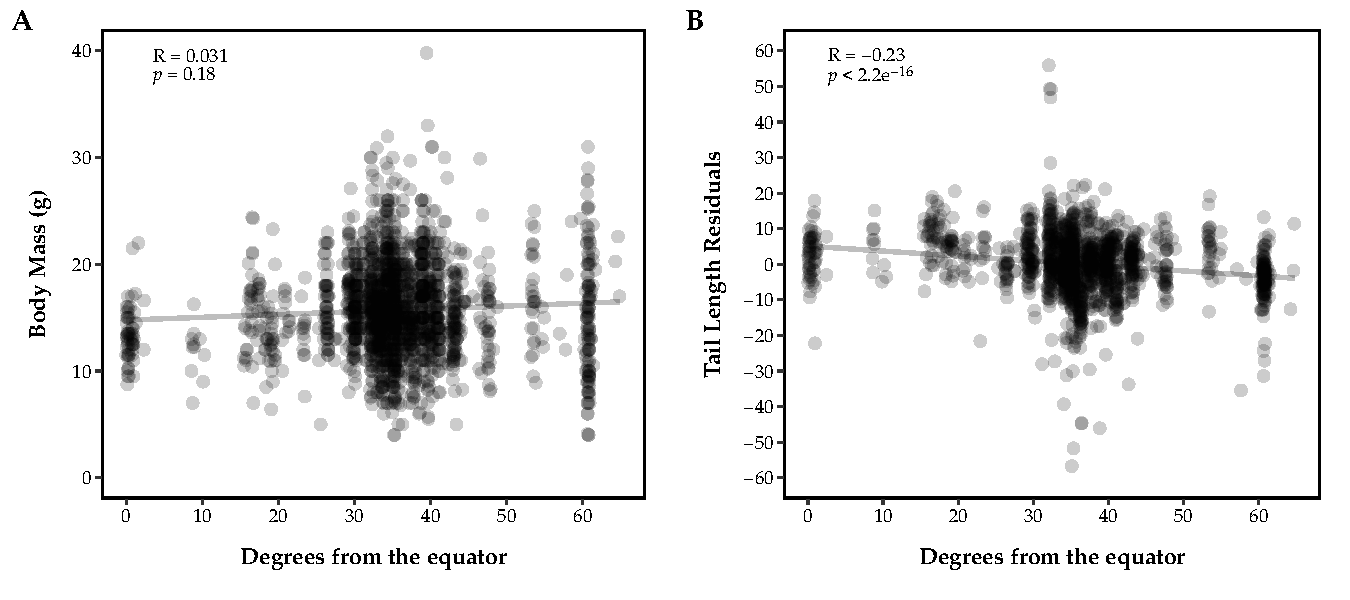
\includegraphics{../figures/VertNet_metadata.pdf}

\textbf{Figure S1. Bergmann's rule and Allen's rule using VertNet
metadata.}

\newpage

\hypertarget{acknowledgements}{%
\subsection{Acknowledgements}\label{acknowledgements}}

\newpage

\hypertarget{references}{%
\subsection{References}\label{references}}

\end{document}
